% !TEX root = ../Rulebook.tex
\section{Scoring} \label{sec:ScoringAndRanking}

For each test the calculation of scores is defined individually, comprising points for achieving certain subtasks and penalty points.

Each test provides a set of so-called feature variations encoding the overall variability of the test (e.g. whether
obstacles can occur or not, number and type of manipulation objects). To enhance comparability among different test
runs, all teams will have to perform the same test instances as specified in Table~\ref{fig:test_specifications_instance}.

For example in a \textbf{perfect} BMT run (perfect means all tasks fulfilled and no penalties given) a team could achieve. This points are calculated using the values out of table \ref{fig:test_scoring}.

\begin{itemize}
	\item 2 Service areas reached: $2 \times 100 = 200$ points
	\item Finish reached: $1 \times 100 = 100 $ points
	\item 3 Objects grasped: $3 \times 100 = 300 $ points
	\item 3 Objects placed: $3 \times 100 = 300  $ points
	\item perfect run bonus: $6 \times 10 = 60 $ points
\end{itemize}

%Explanation of the terms:
%\begin{itemize}
%\item Correct navigating is defined in Section \ref{ssec:Navigating}
%\item Correct grasping is defined in Section \ref{ssec:GraspingObjects}
%\item Correct placing is defined in Section \ref{ssec:PlacingObjects}
%\end{itemize}

\section{Time Bonus}
If a team finishes a test in the required time frame, the left over time will be added as time bonus to the points. 
Time bonus is calculated using the left over time in seconds multiplied by 1. 


\section{Simplifications}
Teams may use simplifications, which will result in a reduction of scores for the given run. The simplifications may be chosen per run, but need to be announced to the referees before the start of the run.


\subsection{Using April Tag Tagged Cubes as Objects}
Real objects are replaced by the April Tag tagged cubes (ATTC)  described in \ref{ssec: April Tagged Object Set}.
Each ATTC is encoded with the matching object ID as defined in the Atwork Commander.
Manipulation tasks count as successful if an atc with a matching object ID is handled correctly. Using this option adds a penalty factor of 50\% to all manipulation points gained.


%\begin{itemize}
%	\item Use of external sensors: \hfill -200 points
%	\item Use of other external objects (e.g. to support localization): \hfill -100 points
%	\item Use of own loading or unloading areas: \hfill -200 points
%  \item Deactivation of Virtual Obstacles (Barrier Tape): -15\% of total points of the run
%\end{itemize}

%Additional simplifications are specified for individual tests. These reductions do not count as penalty points. Teams
%that want to make use of the simplifications above have to announce them in advance of the competition to the TC. The
%TC might forbid the use of specific elements for simplification if these are not in the spirit of the league or may
%cause disproportionate advantages for a team.

\section{Penalties}
\label{sec:penalties}
Penalty points are given as follows, each time again the incident occurs:

\begin{itemize}
	\item Object Loss: \hfill -100 points
	\item Incorrect Object Manipulation (see Section \ref{ssec:PlacingObjects}): \hfill -50 points
	\item Manipulation Deduction (see Section \ref{ssec:PlacingObjects}): \hfill fixed -50 points (for the corresponding grasping or placing)
	\item Minor collision (see Section \ref{sec:Collisions}): \hfill -50 points
	\item Major collision (see Section \ref{sec:Collisions}): \hfill restart or -50\% penalty
  \item Tape collision (see Section \ref{sec:Collisions}): \hfill -5\% of total points of current run up till
  20\%
  \item for each human interaction during the run: \hfill  -100 points
  \item Cheating: \hfill reset all points to 0
\end{itemize}

Manipulation Deduction:

The Manipulation Deduction is a fixed negative point reward (50) if one or more Deductions happen while a grasping or placing process. The type of manipulation (like PP, SH, RT, arbitrary surface etc) when the Deductions happens doesn't affect the fixed points of 50.

\section{Collisions}\label{sec:Collisions}

For reasons of safety of people and property it is strictly unwanted for the robot to collide
with any of the environmental objects. Only collisions of the gripper with the upside of
the service areas are allowed while a Grasping or Placing process. In all collision cases the (Virtual) Walls and Obstacles have an infinite height. The different kind of collisions that can occur are defined in the
following section and the table \ref{tab:collisions} gives an overview. Any Collisions cause a point penalty that is explained in section \ref{sec:penalties}.  

\textbf{Major Collision:}

If the robot (platform and manipulator) collides with a static element of the environment or touches a Virtual Wall it is considered as a major collision. An exception of this rule is when the cables of the manipulator touches the environment while the Grasping or Placing process. As stated before a collision with the  gripper with the upside of the service areas is allowed as long as there is no fundamental change of the environment at the service area. In this case it would be considered as a major collision. This could be for example moving an arbitrary surface off the workspace. 

If a major collision occurs the first time, the team can decide between the following two options:
\begin{itemize}
	\item stop the run and get 50\% of the already reached points
	\item restart the run (the normal restart rules apply)
\end{itemize}
The decision will most likely depend on the remaining run time. If a second major collision occurs, the run is stopped and the team get 50\% of the points reached in the second try.


Since the impact of a major collision on the scoring is very high, the declaration of a major collision is clarified in the following. A major collision is declared by shouting through authorized persons. Nobody is allowed to call a major collision, except the following persons depending on the number of available referees:
\begin{itemize}
	\item only referees, when at least 4 referees (and 1 additional head referee) are available
	\item referees and TC members, when less than 4 referees (without the additional head referee) are available
\end{itemize}
The idea of the two cases is to guarantee a proper number of observers (at least one on each side of the arena). This topic should be highlighted in the referee briefing prior the competition. If a team stops or restarts the run just before the major collision, the major collision is ignored. In this case, the teams knowledge about there robot is rewarded. The referees had to notice that stop or restart was called before the major collision happened. It does not matter whether stop or restart was called before the referees declare a major collision.


\textbf{Minor Collision:}

If the Robot collides with (Manipulation) Objects, Decoys or Containers while moving through the arena it is a Minor Collision. Collisions with Objects, Decoys or Containers while grasping or placing process is considered as Manipulation Deduction.

%If the manipulator collides with an interaction element of the arena (RTT, upper level
%of Shelf) it is considered a minor collision. The only exception is the collision of the gripper
% with the surface of the service area.

\textbf{Tape Collision:}

The yellow/black tape is called Barrier Tape and represents a Virtual Obstacle. If any part of the robot
touches a barrier tape, it is considered a Tape Collision. Tape Collision induce a point penalty
proportional to the final points of the run. With each collision 5\% of the final points are deducted up to a maximum
of 20\%. 

A Collions with the Marking Tape will not be penalized.

%\begin{description}
%  \item[Red/White Tape]: This tape represents a Virtual Wall with an infinitely height. This wall shall not be crossed. If any part of the robot (including the manipulator) is above the tape, it is considered a major collision. 
%  This tape is typically used to limit the area of the arena.
%  \item[Yellow/Black Tape]: This tape is called Barrier Tape and represents a Virtual Obstacle. If any part of the robot
%  touches a barrier tape, it is considered a Barrier Tape Collision. Barrier Tape collision induce a point penalty
%  proportional to the final points of the run. With each collision 5\% of the final points are deducted up to a maximum
%  of 20\%. For beginner teams the option exists to opt-out of Barrier Tape and take a static deduction of 15\% of the
%  final points of the run.
%  \item[Marking Tape]: This tape is used as an universal marker for several purposes and therefore a collision does not matter. 
%\end{description}

\begin{table}[h!]
	\caption{Definition of minor and major collisions}
	\label{tab:collisions}
	\centering
	\begin{tabular}{|p{10cm}|p{1cm}|p{1cm}|p{1.5cm}|}
		\hline
		Situation                                                & Minor & Major &  Tape \\
		\hline
		Collision with static elements of arena                  &       & X     &              \\
		Collision with dynamic elements of arena                 &       & X     &              \\
		Body Collision with WS, SH, RT, PP                     &       & X     &              \\
		Manipulator Collision with top surface of manipulation zone       &       &       &              \\
		Robot Collision with Objecht, Decoy or Container (platform movement)    &  X     &       &              \\

		Manipulator Collision with Shelf                   &      & X      &              \\
		Virtual Obstacle (Yellow/Black Tape) Collisions          &       &       & X            \\
		Virtual Wall (Red/White Tape) Collisions                 &       & X     &              \\
		%Blue/White Tape Collision (1st time gate)                &       &       &              \\
		%Blue/White Tape Collision (2nd time gate)                &       & X     &              \\
		Marking Tape & & & \\
		\hline
	\end{tabular}
\end{table}


\section{Restarts}
Teams might use one so-called restart in a run. Scores achieved before the restart are set to zero. Please refer to section \ref{sec:restartingarun} for a more detailed explanation.
%\begin{itemize}
%	\item Self called: Scores that are received after a restart are not reduced.
%	\item Major collision: Scores that are received after a restart are reduced with multiplication of 0.75.
%\end{itemize}

\section{Ranking}
The tests will occur in the instances shown in Table~\ref{fig:test_specifications_instance}. Ranking of the teams will be based on the sum of the achieved points over all the tests.

A team cannot get less than zero points for one run. If it is necessary to divide the competition into two stages (see section ~\ref{sec:qulaification for a test}), the scores of the first stage tests are summed up, and the teams with the highest sums proceed to the next stage (depending on overall number of teams). Depending on the number of teams and if there is enough time, all teams are allowed to enter the second stage.

In case of a tie of the first three places a deciding run will be scheduled. A point tie down from 4th place will result in to sharing the achieved place. 


%\setlength{\tabcolsep}{4.75pt}
%\renewcommand{\arraystretch}{1.1}
%\newcommand{\R}[2]{
%	\begin{turn}{90}
%		\begin{minipage}[][1em][c]{#2}
%		#1
%	  \end{minipage}
%	\end{turn}
%}
%
%\newcommand{\cir}[1]{\hspace{0.5em}\unitlength1ex\begin{picture}(2.8,2.8)%
%\put(0.75,0.75){\circle{2.8}}\put(0.75,0.75){\makebox(0,0){#1}}\end{picture}}
%\newcommand{\Y}{\tiny \CIRCLE}
%\newcolumntype{P}[1]{>{\centering\arraybackslash}p{#1}}
%
%\definecolor{headlineColor}{rgb}{.7,.7,.7}
%\definecolor{sectionColor}{rgb}{.7,.1,.1}
%
%\newcommand{\C}{\cellcolor{sectionColor}}


%\begin{landscape}
%\begin{table}
% \centering
% \begin{tabular}{|p{5.5cm}*{9}{|P{1cm}}|}
%   \hhline{~--------}
%   \multicolumn{1}{l|}{}                       & \multicolumn{8}{c|}{Instances}                               \\
%   \hhline{~--------}
%   \multicolumn{1}{l|}{}                       &\cir{1} &\cir{2} &\cir{3} &\cir{4} &\cir{5} &\cir{6} &\cir{7} \\
%   \multicolumn{1}{r|}{}                       & BMT    & BTT1   & BTT2   &  BTT3  & PPT    &  RTT   & Final  \\
%   \hhline{~--------}
%   \hline
%	 Correct service area reached                &   25   &   25   &  25    &   25   &  25    &   25   &   25   \\ \hline
%   Correct object grasping           &    &    &     &    &     &        &    \\
%     \hspace{0.5cm} standard            &  100   &  100   & 100    &  100   &   0    &        &  100   \\
%	 \hspace{0.5cm} round table                  &        &        &        &        &        &  300   &  200   \\
%	 \hspace{0.5cm} PPT area                     &        &        &        &        &        &        &  200   \\
%	 \hspace{0.5cm} arbitrary surface (tbdiscussed... reduce points)           &        &  150   & 150    &  150   &        &        &  150   \\
%	 \hspace{0.5cm} shelf upper level            &        &        &        &  150   &        &        &  150   \\
%	 \hspace{0.5cm} shelf lower level            &        &        &        &  300   &        &        &  300   \\ \hline
%   Correct object placing standard (tbdiscussed... increase, more than grasping to motivate the teams to implement placement with collision avoidance?)            &   75   &   75   &   75   &   75   &        &        &   75   \\
%	 \hspace{0.5cm} PPT area                     &        &        &        &        &  200   &        &  200   \\
%	 \hspace{0.5cm} shelf upper level            &        &        &        &  150   &        &        &  150   \\
%	 \hspace{0.5cm} shelf lower level            &        &        &        &  150   &        &        &  150   \\ \hline
%   Incorrect object placing tbdiscussed... (wrong service area?)                   & -100   & -100   & -100   & -100   & -100   &        & -100   \\
%	Incorrect object placing tbdiscussed... (outside manipulation zone and/or touching other objects)                    & 50   & 50   & 50   & 50   & 50   &        & 50   \\
%   Incorrect object grasping                   &        & -100   & -100   & -100   &        & -100   & -100   \\
%   Completing whole task                       &   75   &  100   &  150   &  250   &   50   &   75   &  300   \\ \hline\hline
%   Maximum attainable points\newline (time bonus not included)
%	                                             & 1000   & 1100   & 1400   &  2000  &  700   &  1000  &  3200  \\ \hline
% \end{tabular}
% \caption{Scoring in the instances of the \RCAW \YEAR competition.}
%  \label{tab:InstancePoints}
%\end{table}
%\end{landscape}


\begin{figure}[h!]
	\centering
	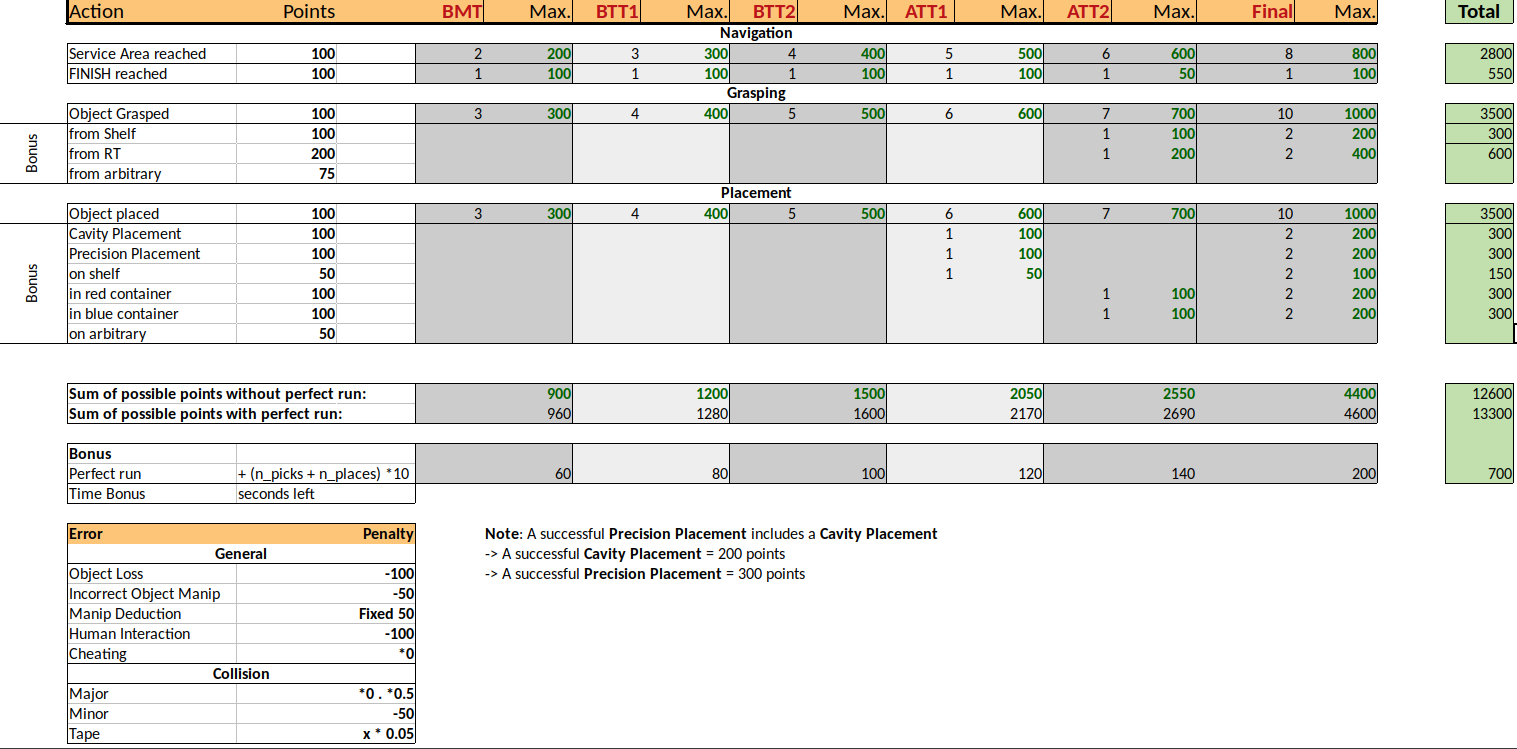
\includegraphics[width= 1\textheight, angle=90  ]{./images/tabels/robocup_penalty_points.png}
	\caption{Scoring in the instances of the \RCAW \YEAR competition.}
	\label{fig:test_scoring}
\end{figure}
